\begin{figure}
\centering
\begin{subfigure}{\columnwidth}
  \centering
  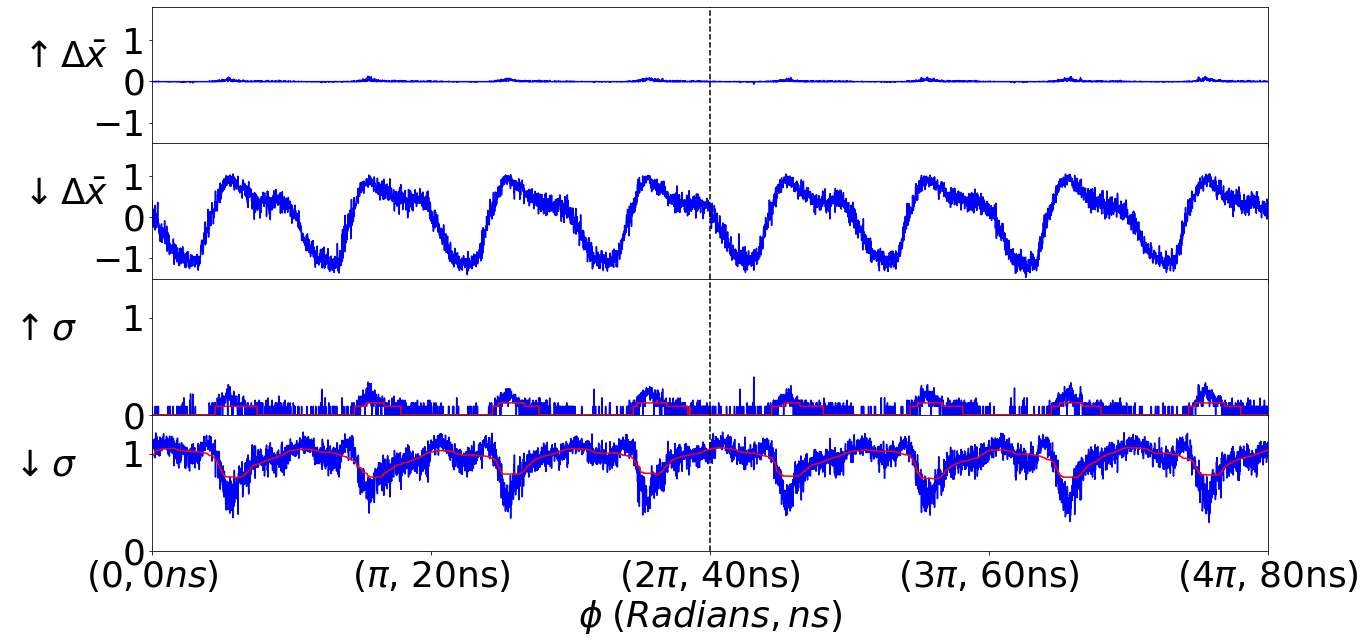
\includegraphics[width=\linewidth]{img/Base_pynq_std_ham_pn_4pi.png}
  \caption{PYNQ-Z2 Baseline Hamming Distance Rising($\uparrow\bar{x}$) and Falling($\downarrow\bar{x}$), Standard Deviation Rising($\uparrow\sigma$) and Falling($\downarrow\sigma$) \cd{maximize foe each edge}}
%  \caption{Baseline (Falling Transition)}
  \label{fig:phi-base}
\end{subfigure}
\bigskip
\vspace{-10pt}
\centering
\begin{subfigure}{\columnwidth}
  \centering
  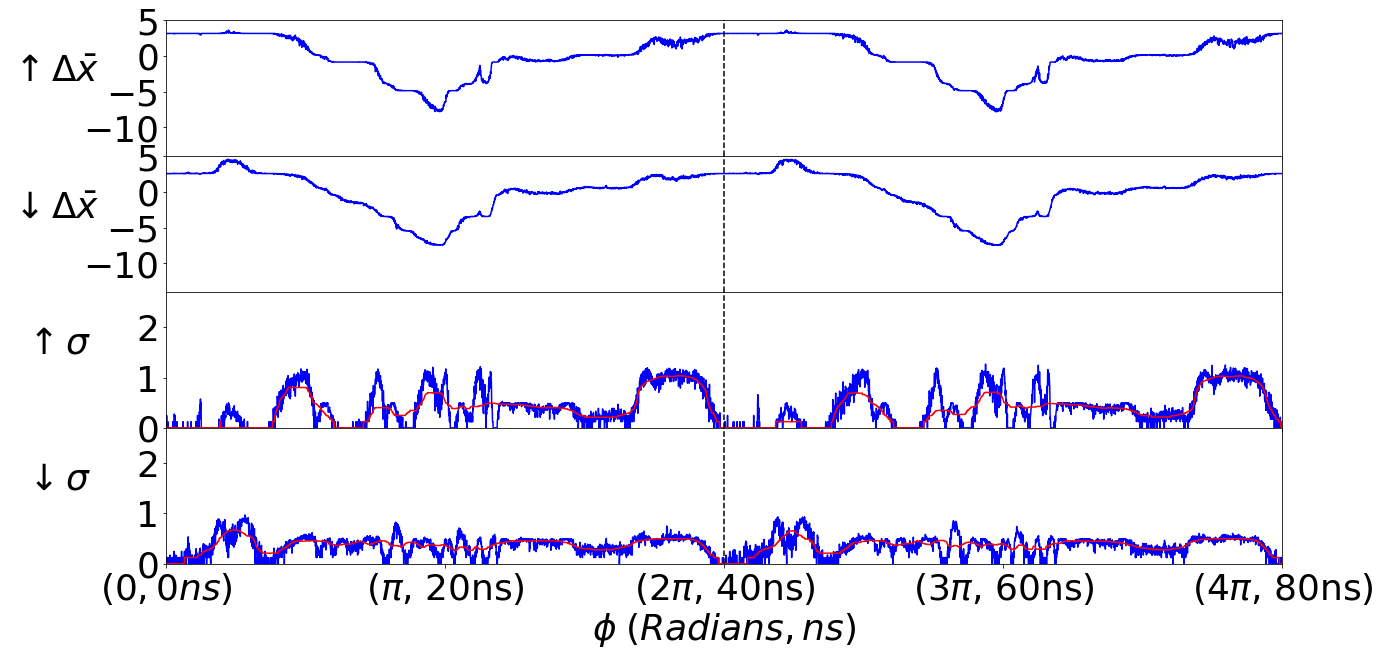
\includegraphics[width=\linewidth]{img/DSP_pynq_std_ham_pn_4pi.png}
  \caption{PYNQ-Z2 DSP Hamming Distance Rising($\uparrow\bar{x}$) and Falling($\downarrow\bar{x}$), Standard Deviation Rising($\uparrow\sigma$) and Falling($\downarrow\sigma$)}
%  \caption{Baseline (Falling Transition)}
  \label{fig:phi-base}
\end{subfigure}
\label{fig:phi-shift}
\caption{PYNQ-Z2 phi sweeps}
\end{figure} 
